% !TEX root = base.tex 

\chapter{Hematite Film Reactivity on Polycrystalline Substrates}
\label{ch:polycrystalline.reactivity.old}


This chapter presents results photochemical activity for \ce{Fe2O3} films deposited on polycrystalline \ce{BaTiO3} substrates. \ce{BaTiO3} was selected as the substrate material for its ferroelectric properties. Film growth and orientation relationships were analyzed using electron backscatter diffraction mapping. Photochemical activity under visible and ultraviolet illumination was tested using the marker reaction of the reduction of aqueous silver to solid silver. For comparison with results on single crystal \ce{SrTiO3} substrates, a polycrystalline \ce{SrTiO3} pellet would be the obvious choice of substrate. However, photochemical properties were the primary driver of this investigation, leading to the choice of \ce{BaTiO3}. \ce{SrTiO3} and \ce{BaTiO3} are closely related in structure and properties. For the purposes of the determination of orientation relationships, the system of \ce{BaTiO3} and \ce{Fe2O3} is expected to behave the same as \ce{SrTiO3} and \ce{Fe2O3}.


\section{Experimental Details}
\label{sec:ch6experimental}


Polycrystalline \ce{BaTiO3} pellets were prepared as described in Chapter \ref{ch:experimental}. \ce{Fe2O3} films were deposited on these substrates following the procedures described in Chapter \ref{ch:experimental} for pulsed laser deposition. For film growth analysis, the film thickness was \SI{180}{\nano\meter} to ensure EBSD signals were representative the film, rather than the substrate. For photochemical activity measurements, the same \SI{180}{\nano\meter} thick film sample was used, as well as \SI{60}{\nano\meter} and \SI{7}{\nano\meter} thick films on different \ce{BaTiO3} pellets.


\section{Film Growth on Polycrystalline Barium Titanate}
\label{sec:ch6filmgrowth}


\subsection{EBSD Analysis}
\label{subsec:ch6ebsd}


Electron backscatter diffraction was used to determine the orientation relationships for \ce{Fe2O3} films deposited on polycrystalline \ce{BaTiO3} substrates. \ce{BaTiO3} pellets were prepared, polished, and annealed as described in the experimental section of this document. Prior to film deposition, and electron backscatter diffraction was used to map the orientation of the BTO substrate grains. After film deposition, the same area of the sample was mapped again with EBSD. Figure \ref{fig:orientationmaps} shows orientation maps of the same area of the sample before and after film deposition.%
\begin{figure}
	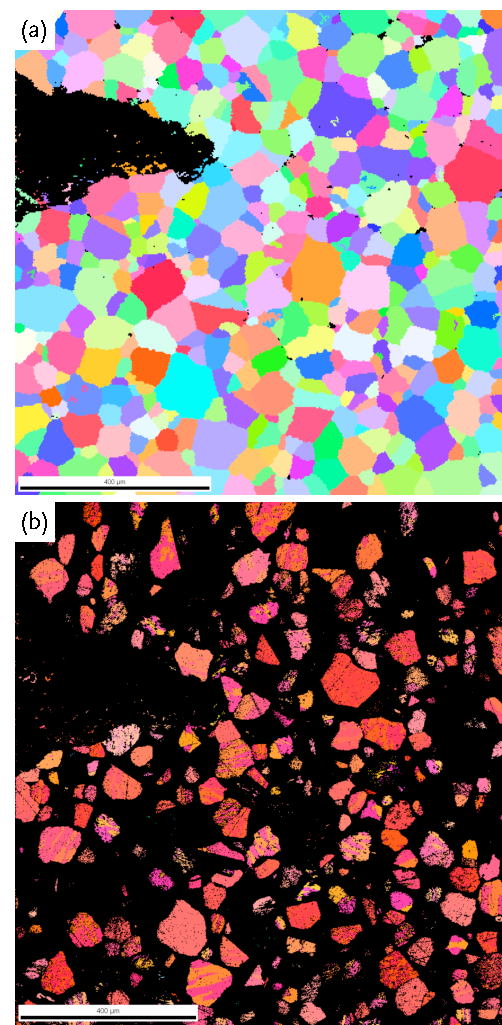
\includegraphics[width=0.8\textwidth]{orientationmaps.pdf}
		\caption[EBSD maps of substrate and film]{%
			a) EBSD inverse pole map of a polycrystalline \ce{BaTiO3} substrate. 
			(b) EBSD inverse pole map of the same area of the sample after 
			\ce{Fe2O3} film deposition. Black points represent points of low 
			confidence index and pattern quality.}
	\label{fig:orientationmaps}
\end{figure}
The large area of black, unindexed points in the substrate map corresponds to a large crack in the sample. This crack was used as a fiduciary mark to assist in relocating the same area of the sample, and for alignment of the two orientation maps. The substrate EBSD data was processed with one iteration of a grain dilation algorithm, and subsequently assigning a single average orientation to each grain. In the grain dilation cleanup method, points not belonging to an already identified grain (based on misorientation angle and grain size) are changed to the orientation of the nearest grain.  For this procedure, the minimum grain size was 5 pixels and the grain tolerance angle was 5\si{\degree}. The grain averaging procedure uses a tolerance angle to identify grains, and then assigns a single orientation to that grain, averaging the orientation of all points within the identified grain. The results of these two cleanup procedures are a map with clearly identified grains of a single orientation. Manual inspection of the orientation map shows that the identified grains of the map correspond to the size and shapes of grains as viewed through an optical microscope. Because the sample was annealed after polishing, the grain boundaries are grooved, and clearly visible in the optical microscope. Because each grain now has a single orientation, it is possible to use this angle to calculate the misorientation between the substrate grain and its corresponding film grain. The grain tolerance angle while assigning a single orientation to each grain was 5\si{\degree}. The film scan only shows points that were indexed with a high degree of certainty, according to the EBSD software. These points were partitioned by manually selecting a minimum pattern image quality value. All of the points visible on this map had a significantly higher image quality value than the points appearing as black on this map. Before partitioning, the, dataset was cleaned using the same grain dilation and average orientation algorithms as for the substrate. 

Film grains demonstrate (0001) texture. All film grains that were indexed with high confidence by the automated software are oriented near the (0001) orientation, and appear as red, orange, or pink on the inverse pole map. Figure \ref{fig:overlaymap} shows the two maps overlaid, illustrating the alignment of film grains on substrate grains. 
\begin{figure}
	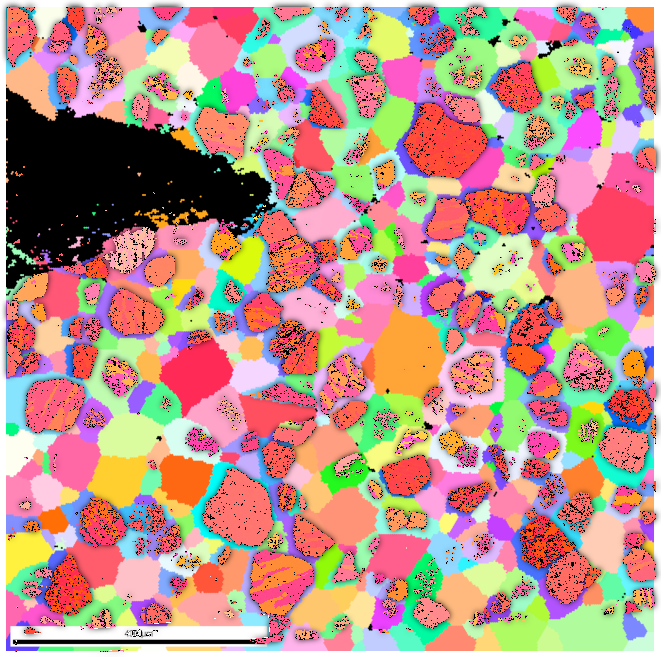
\includegraphics[width=\textwidth]{overlaymap.pdf}
		\caption[Film and substrate maps overlaid]{%
			Film and substrate maps overlaid, showing the correlation 
			between film grains and substrate grains.}
	\label{fig:overlaymap}
\end{figure}
This shows the correlation between the areas of indexed film grains and the substrate grains. In most cases, it is possible to establish a relationship between film grains and their corresponding substrate grains. For many substrate grains, multiple film grains are supported on the single substrate grain. For these film grains, it is observed that all the grains supported on a single substrate grain share a common set of Miller indices (hkil), with different permutations of the first three being responsible for the differing orientation. This suggests that the multiple film grains exist as twins on the single substrate grain.

The points on the inverse pole figure seen in Figure \ref{fig:polyipfs}(a) represent the substrate grains on which film grains were identified. The corresponding film grains are shown in Figure \ref{fig:polyipfs}(b).
\begin{figure}
	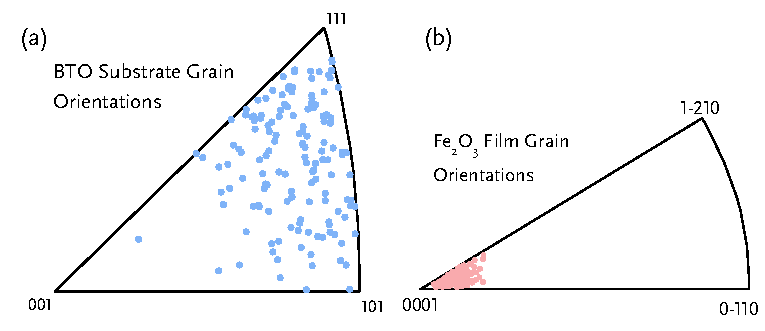
\includegraphics[width=\textwidth]{polyipfs.pdf}
		\caption[Orientations of film and substrate grains]{%
			(a) Each point on this inverse pole figure represents the orientation of a \ce{BaTiO3} substrate grain that nucleated epitaxial film grains. (b) Each point on this inverse pole figure represents the orientation of an \ce{Fe2O3} film grain.}
	\label{fig:polyipfs}
\end{figure}
These inverse pole figures show the already observed preference for film grains to be oriented near the (0001) direction. What wasn't clear from a preliminary inspection of the orientation maps is the preferred orientation of the substrate grains. The only substrate grains which promoted the growth if indexable film grains were located away from the cubic (001) direction. Grains located near (111) or (110) orientations were much more likely to correspond to identified film grains. Given the previously observed behavior of films grown in single crystal substrates, this is not entirely surprising. In the single crystal case, epitaxial films of (0001) orientation were grown on (111) oriented \ce{SrTiO3} substrates. On single crystal (001) substrates, textured polycrystalline \ce{Fe2O3} films were formed. In the case of the polycrystalline substrate however, no clear film grains were indexed on substrate grains near the (001) orientation. A possible explanation for the difference in behavior lies in the different surface quality of the polycrystalline substrate as compared to the single crystal. The polycrystalline surface is considerably rougher than the surface of the single crystal. Facets, pores, and steps exist on the surface of the polycrystal. As a result surface diffusion of atoms during the deposition process is expected to be much lower. This changes the nucleation and growth of the film on the polycrystal, possibly resulting in grains that are much smaller than on single crystals. These small grains are considerably more difficult to index during EBSD, especially in the automated process.

\subsection{Orientation Relationship Calculations}\label{subsec:ch6orientations}

In the case of film growth on the polycrystal, many of the grains which formed films were tilted away from (111). Yet these grains still show single crystal films. For \ce{Fe2O3} films on single crystal \ce{SrTiO3} (001) substrates, the \ce{Fe2O3}(0001)||\ce{SrTiO3}(111) orientation relationship persisted, even though the \ce{BaTiO3} (111) direction was not the out of plane direction. It was hypothesized that a similar relationship could be determined for the substrate grains tilted away from the (111) direction on the polycrystalline substrate. The \ce{Fe2O3}(0001)||\ce{SrTiO3}(111) orientation relationship would persist, even for grains tilted away from (111) orientation. To test this hypothesis, data from these maps was exported in the form of a text file containing a single line for each identified grain of the scan. Each grain was assigned a unique number ID. This ID was included, along with the Euler angles corresponding to the angle of that grain.  The grain ID for each film grain was manually paired with the grain ID for its corresponding substrate grain. This was done through visible inspection of the overlaid maps depicted in Figure \ref{fig:overlaymap}. Only film grains that could clearly be assigned to a substrate grain were included in the pairing list. Because multiple film grains exist on a single substrate grain, in many cases multiple pairing exist for a single substrate grain. A Fortran program \sidenote{Developed by Gregory S. Rohrer.} was then used to calculate the minimum angle between a film direction and a substrate direction, taking into account symmetry operations for the crystal structure of the film and substrate. 

When the angle between the substrate [111] direction and the film [0001] direction is calculated for the 399 identified pairs in these scans, the average angle between the substrate [111] and the film [001] is 2.4\si{\degree}, well within the experimental variance of the EBSD technique. The same orientation program was used to calculated the angle between the substrate [110] direction and the film [210] direction. For this relationship, the average misorientation was 1.7\si{\degree}. These directions were chosen because they are both located in the basal plane of the film and the (111) plane of the substrate. They serve as directions for ``in plane'' alignment, even when they are no longer in the plane of the sample surface. Figures \ref{fig:inplane} and \ref{fig:outofplane} show the distribution of the misorientation angles for these two pairs of directions. 
\begin{figure}
	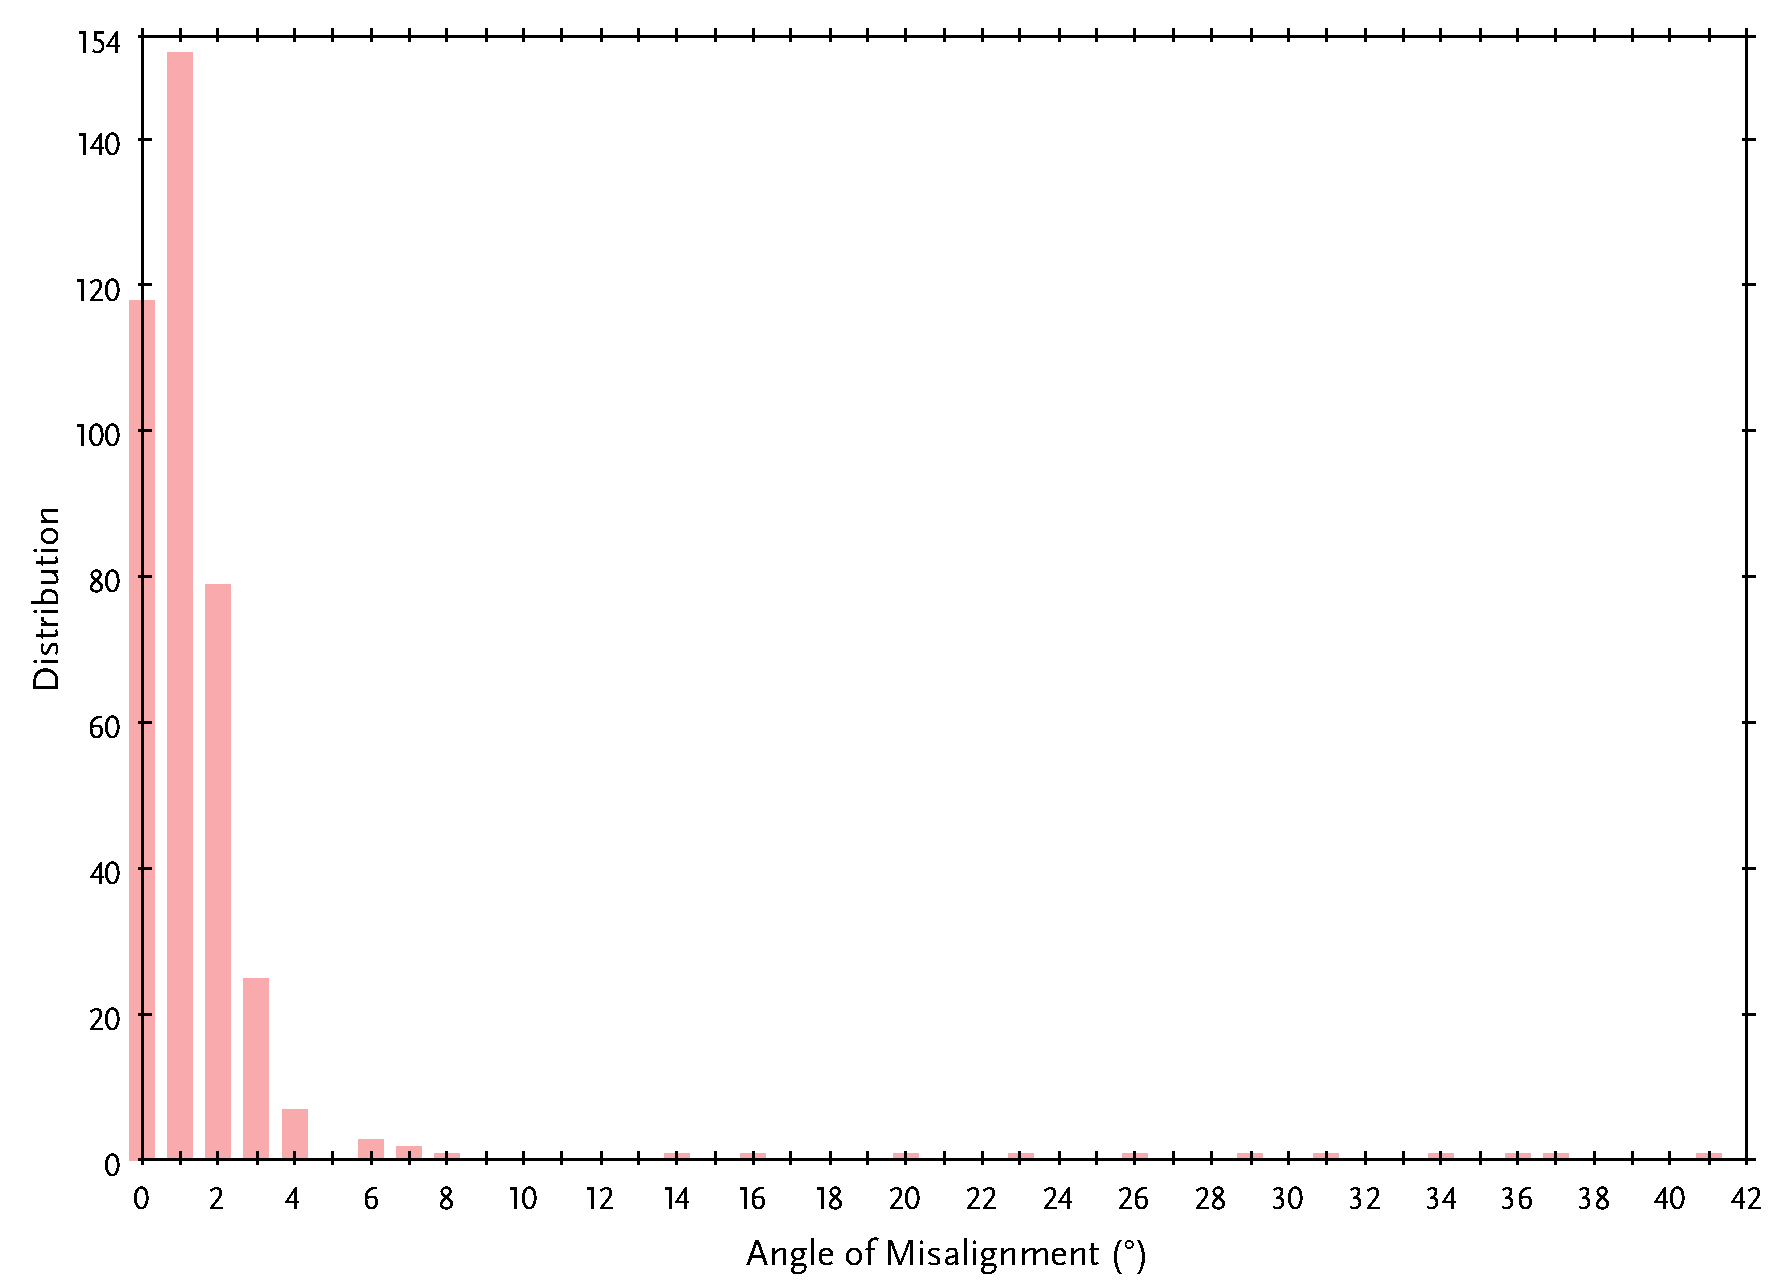
\includegraphics[width=\textwidth]{outofplane.pdf}
		\caption[Distribution of out of plane misalignment]{%
			Distribution of out of plane misalignment between the 
			substrate (111) direction and the film (001) direction 
			for the points depicted in Figure \ref{fig:polyipfs}.}
	\label{fig:outofplane}
\end{figure} 
\begin{figure}
	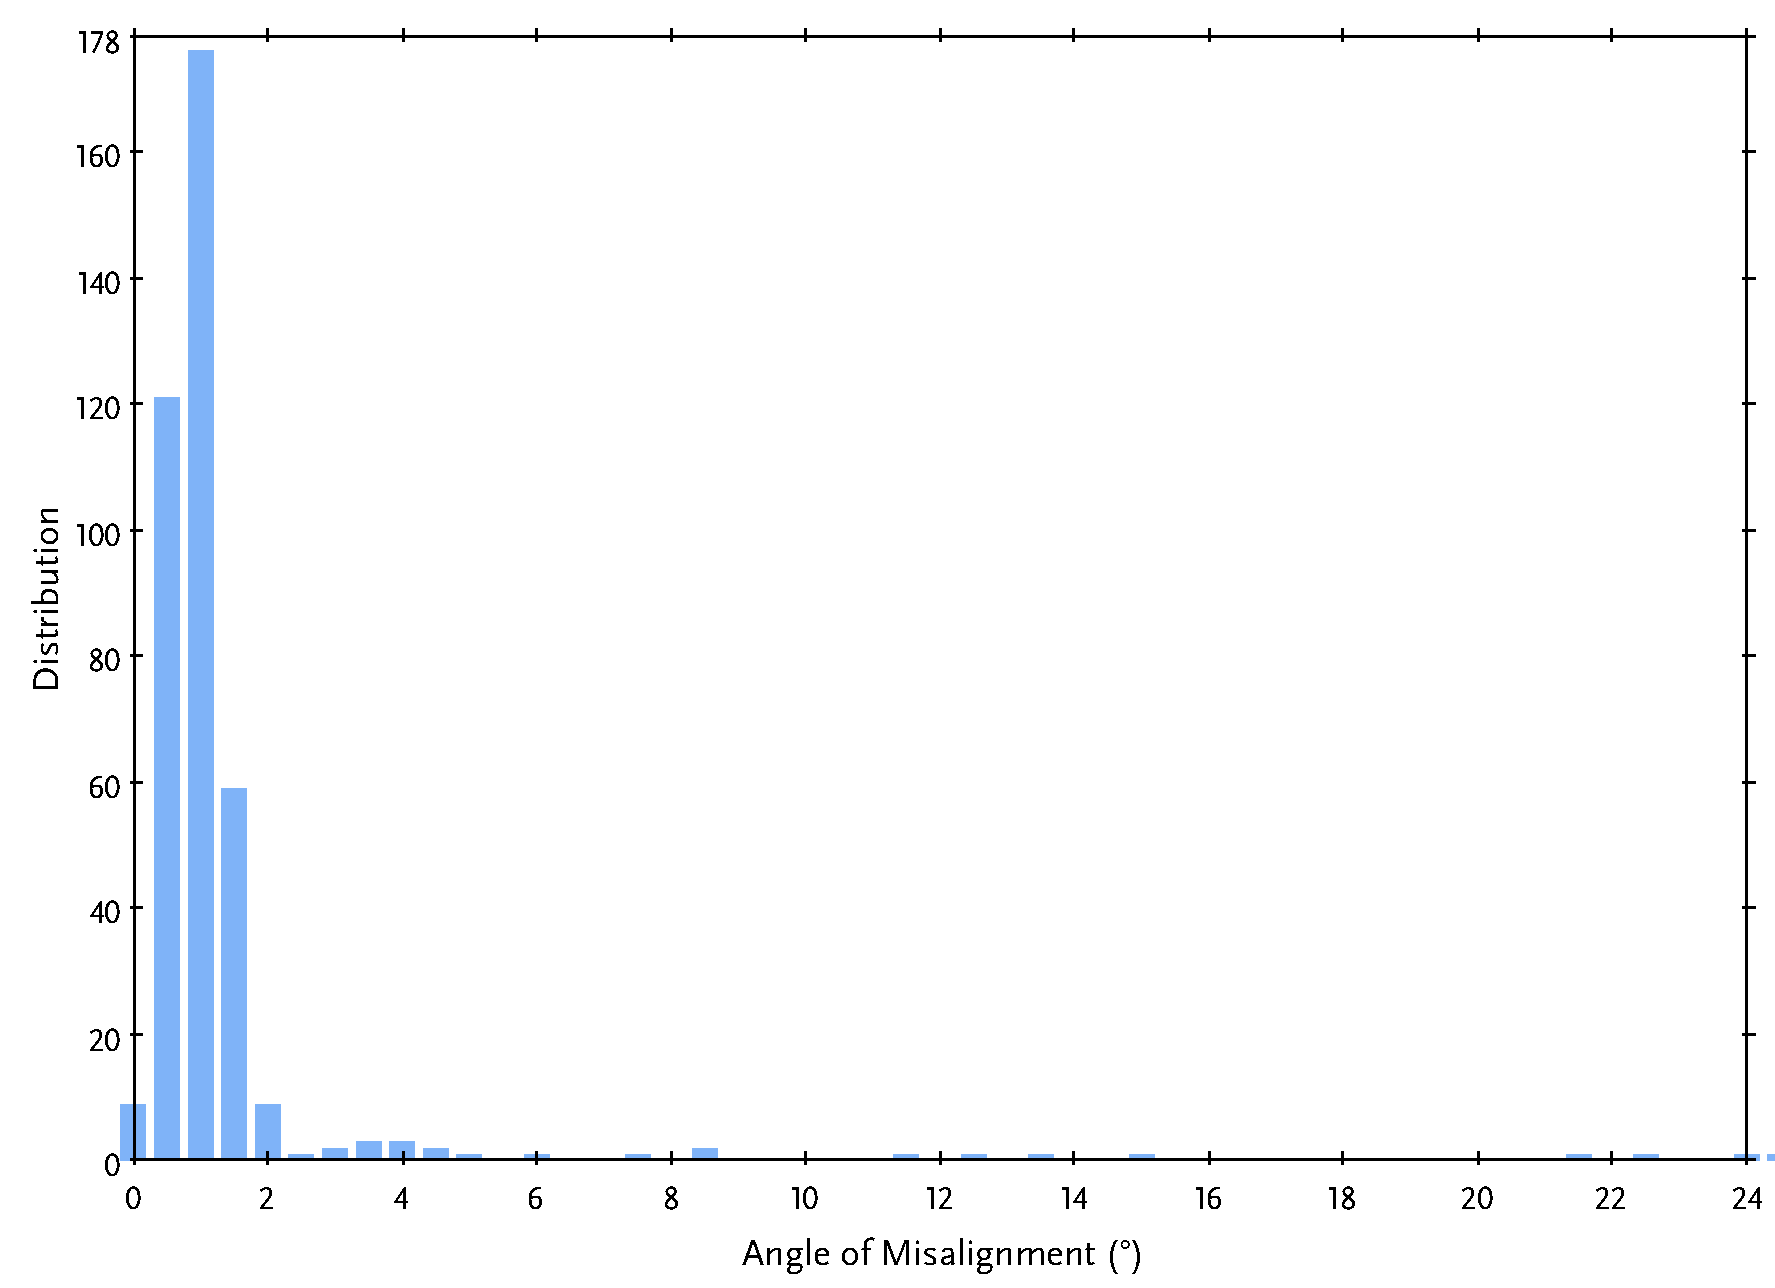
\includegraphics[width=\textwidth]{inplane.pdf}
		\caption[Distribution of in plane misalignment]{%
			Distribution of in plane misalignment between the 
			substrate (110) direction and the film (210) direction 
			for the points depicted in Figure \ref{fig:polyipfs}.}
	\label{fig:inplane}
\end{figure}
In most cases, the c-axis of the hexagonal film is directly in line with the [111] axis of the cubic substrate. As the [111] substrate direction tilts away from being perfectly normal to the surface, the film c-axis tilts by the same orientation. Not only did the c-axis of the film align with the [111] direction of the substrate, even when that direction was tilted far away from normal to the sample surface, but alignments orthogonal to the c-axis also persisted.  


\section{Reactivity Results for Films on Polycrystalline Substrates}\label{sec:ch6reactivity}


\subsection{Domain-selective Reactivity}
\label{subsec:ch6domain}


Earlier work studying the photochemical activity of thin titania films supported on ferroelectric substrates has shown that photochemical reaction with aqueous salts occurs on spatially selective regions of the film surface, corresponding to the ferroelectric domains of the substrate. [15,21,22] Burbure [15] attempted to qualitatively describe the band structure of these heterostructures, and the resulting band diagrams are depicted in Figure \ref{fig:ninabending}. 
\begin{figure}[htbp]
\begin{center}
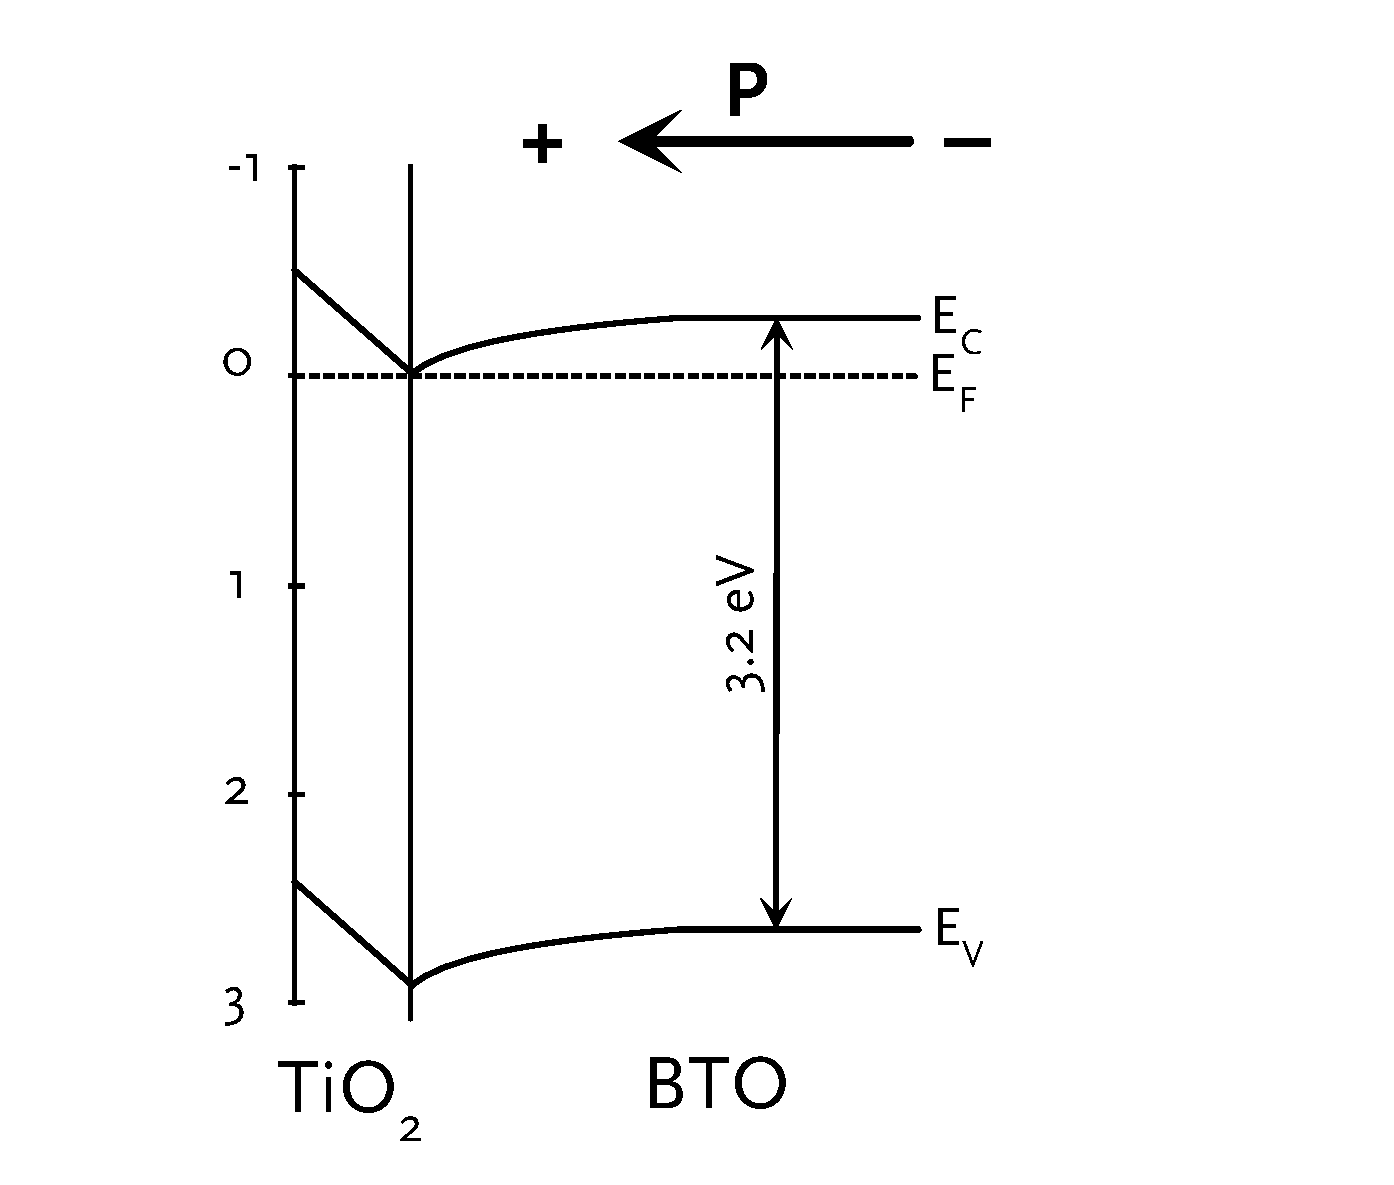
\includegraphics[width=0.4\textwidth]{ninabending.pdf}
\caption[Proposed band bending of a \ce{TiO2}/\ce{BaTiO3} heterostructure]{Schematic showing the proposed band bending of a \ce{TiO2}/\ce{BaTiO3} heterostructure owing to the ferroelectric \ce{BaTiO3} substrate. [15]}
\label{fig:ninabending} % 6.6
\end{center}
\end{figure}
Burbure proposed that the band bending in the substrate arising from the ferroelectric field is responsible for driving charge carriers in opposite directions, and that domains of opposite polarization will drive opposite charge carriers to the surface of the film. The film material was assumed to be too thin to allow for total equilibrium between the film bands, the substrate bands, and the solution. The scheme in Figure \ref{fig:ninabending} suggests that charge carriers in the film experience an electric field in the opposite direction of the field experienced in the substrate. It was assumed that the charge carriers reaching in the film would arrive with enough energy to reach the surface of the film. But the question of what happens to charge carriers generated in the film remains. The scheme in Figure \ref{fig:ninabending} suggests that if charge carriers were generated solely in the film material, domain-selective reactivity would persist, but would occur on domains of the opposite polarization. In the \ce{TiO2}/\ce{BaTiO3} system, this effect couldn't be tested. Because the film is so thin, it is stated that the majority of the charge carriers involved in photochemical reaction are generated in the substrate. Additionally, the band gaps of the substrate (\texttildelow\SI{3.2}{\electronvolt}) and film (\texttildelow\SI{3.0}{\electronvolt}) materials were too similar to use optical filters to prevent charge carriers from being generated in the substrate. 

The use of \ce{Fe2O3} as a film material presents the opportunity to overcome those limitations, and test the photochemical behavior of charge carriers generated in the film. Under the visible light illumination used for earlier photochemical experiments, charge carriers would only be generated in the film of an \ce{Fe2O3}/\ce{BaTiO3} heterostructure. The band gap of the substrate is too large for the absorption of blue light to excite an electron from the valence band to the conduction band. The marker reaction of the reduction of aqueous silver was used to test the spatial selectivity of reaction for charge carriers generated in the visible light absorbing film.

A 60 nm hematite film was deposited on a polycrystalline \ce{BaTiO3} substrate. The substrate was prepared, polished, and annealed as described in the experimental chapter (\S \ref{sec:ch3pld}) of this document. Deposition procedures and conditions were the same as described previously for the growth of \ce{Fe2O3} films. Figure \ref{fig:btoblue} shows the AFM micrographs surface of the film after the photochemical marker reaction with \ce{AgNO3} under blue LED illumination. 
\begin{figure}[htbp]
\begin{center}
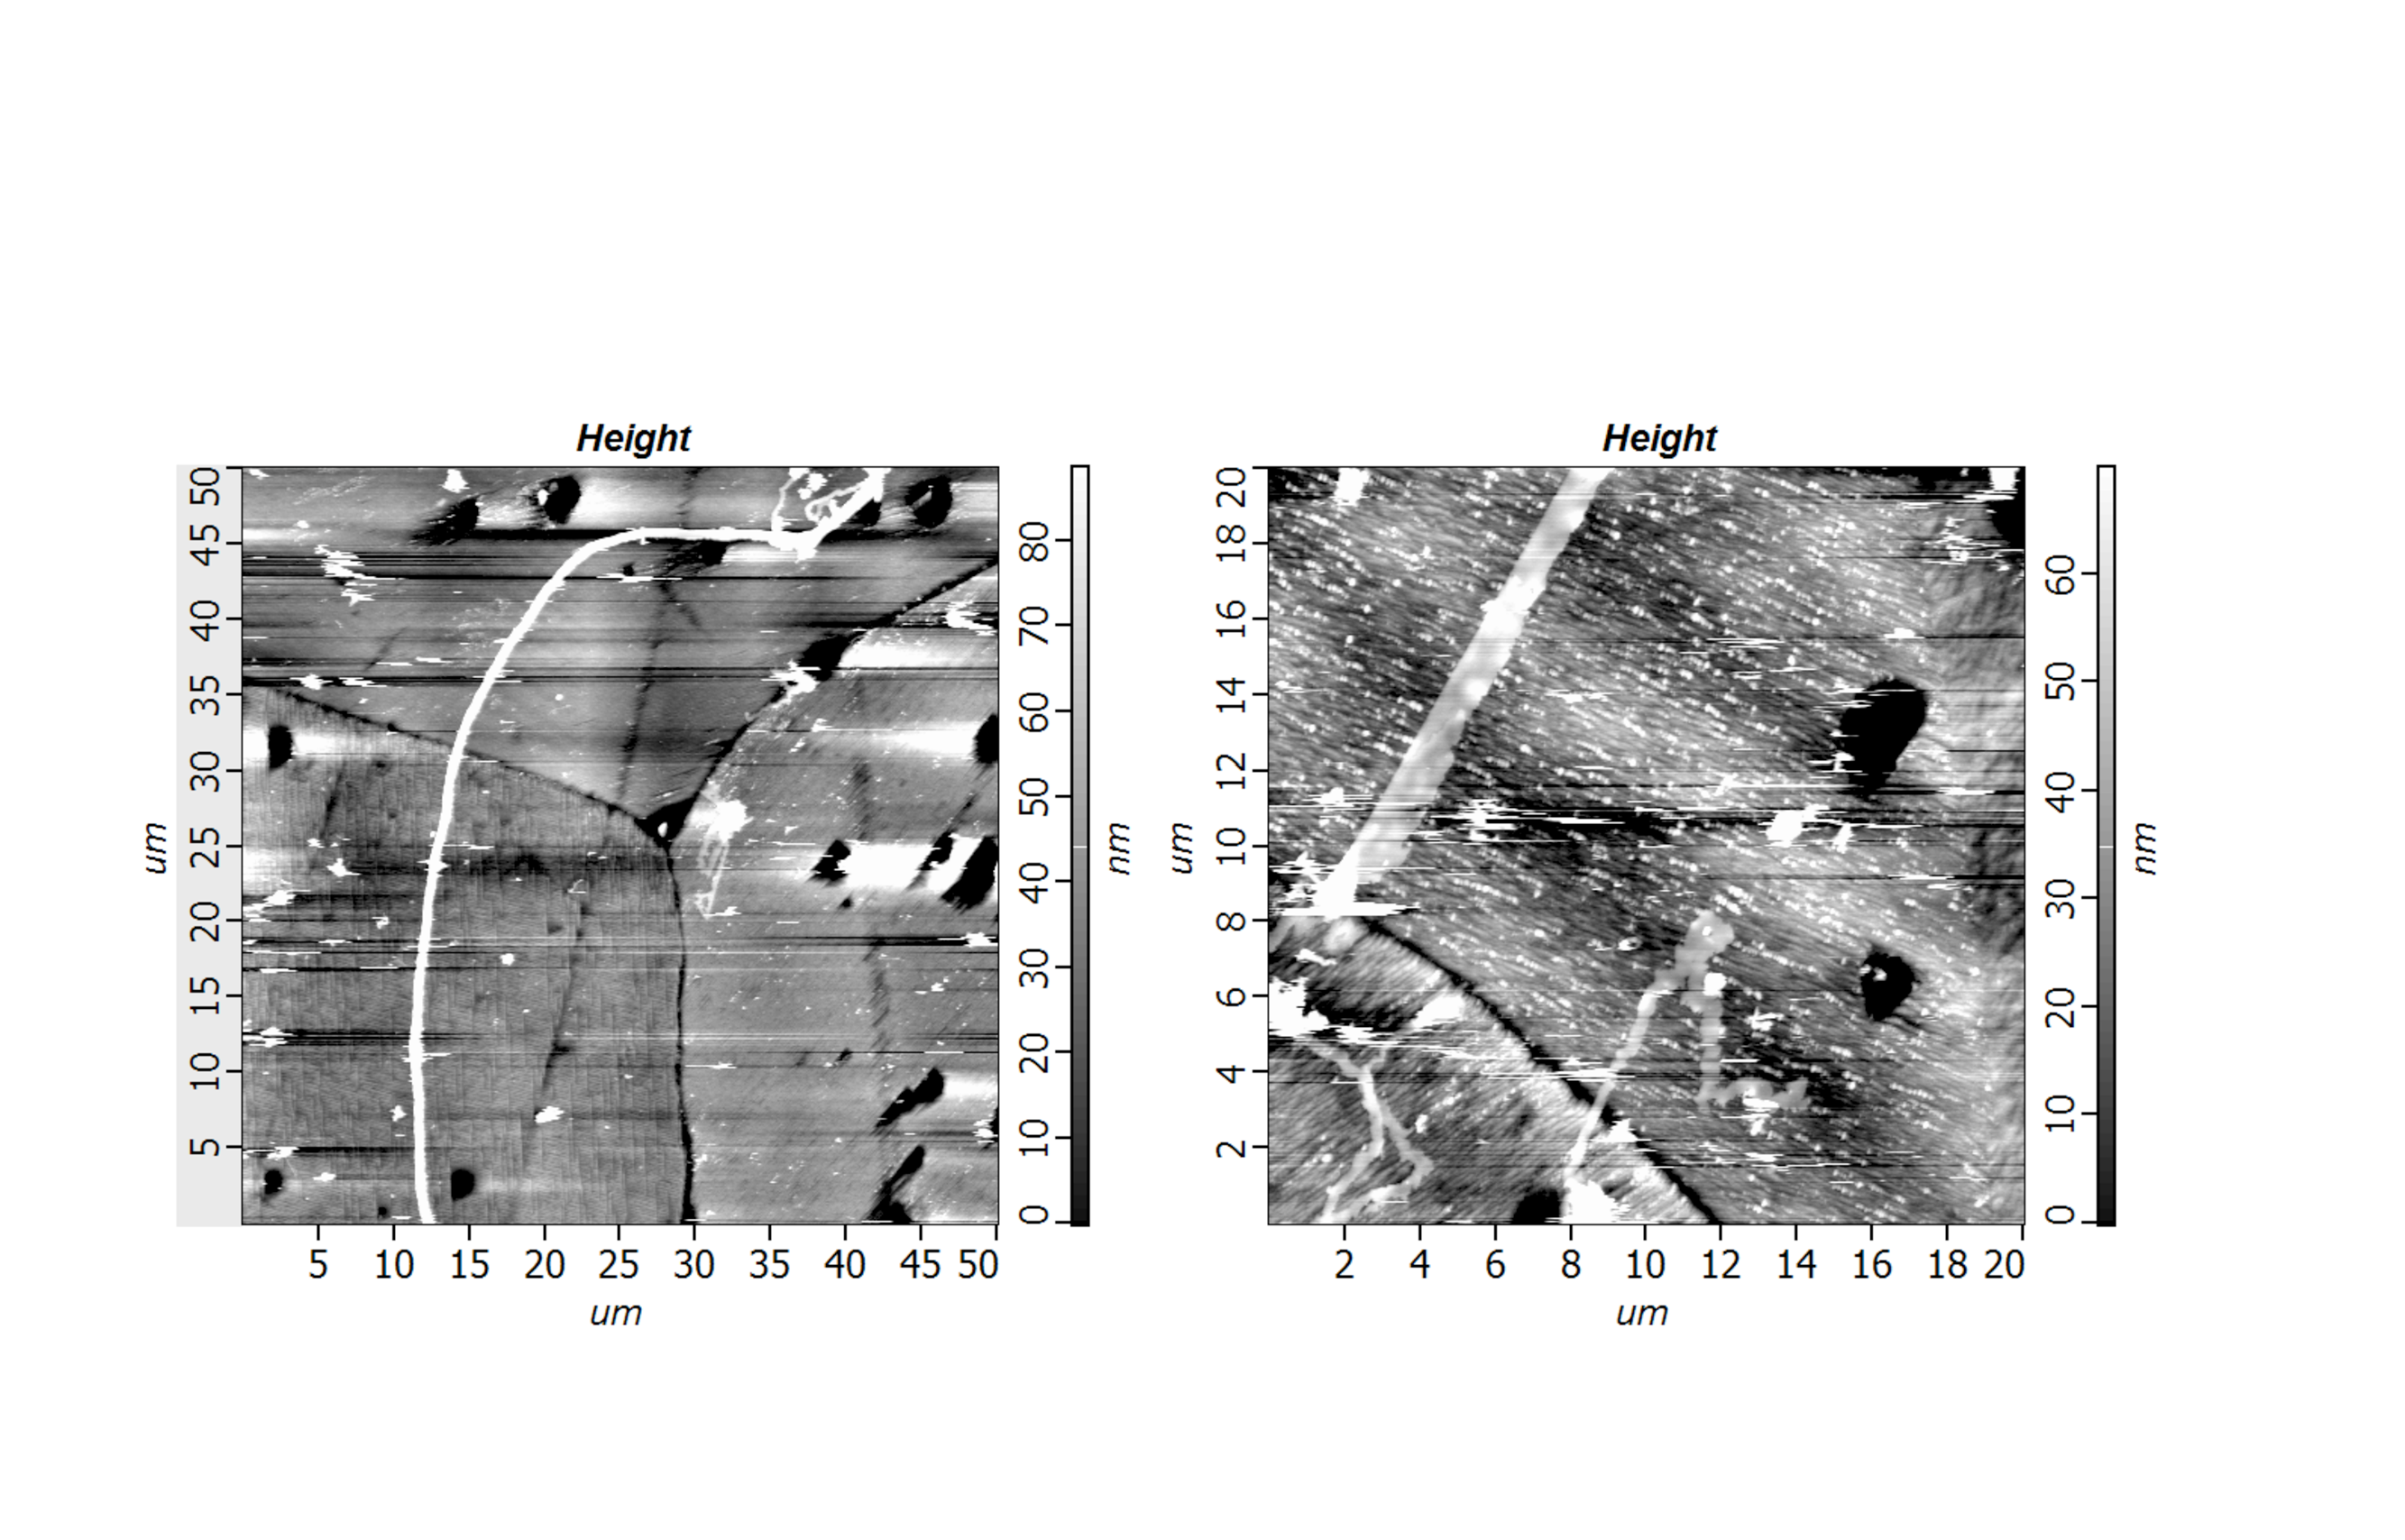
\includegraphics[width=\textwidth]{btoblue.pdf}
\caption[Surface of an \ce{Fe2O3} film on \ce{BaTiO3} after reaction]{Surface of an \ce{Fe2O3} film on \ce{BaTiO3} after reaction with \ce{AgNO3} solution under visible light illumination. No patterns corresponding to the ferroelectric domains of the substrate are observed.}
\label{fig:btoblue} % Figure 6.7
\end{center}
\end{figure}
Illumination time was \SI{30}{\minute}, and the current through the LED was \SI{500}{\milli\ampere}. Unlike the \ce{TiO2}/\ce{BaTiO3} heterostructures, the reaction product on the surface of \ce{Fe2O3} films on \ce{BaTiO3} substrates do not appear in patterns corresponding to the ferroelectric domains of the substrate. This was true for all examined grains of the sample. This suggests that under visible light illumination, when charge carriers are only generated in the film, spatially selective reactivity does not occur.

The selectivity of photochemical reactions on \ce{Fe2O3}/\ce{BaTiO3} heterostructures under ultraviolet illumination was also tested. Under UV light, the majority of the charge carriers are expected to be generated in the substrate, and the behavior of the heterostructure is expected to be similar of that of \ce{TiO2} films on \ce{BaTiO3} substrates. AFM scans of the surface of the \SI{7}{\nano\meter} thick film before and after reaction under UV light are shown in Figure \ref{fig:btouv}.
\begin{figure}[htbp]
\begin{center}
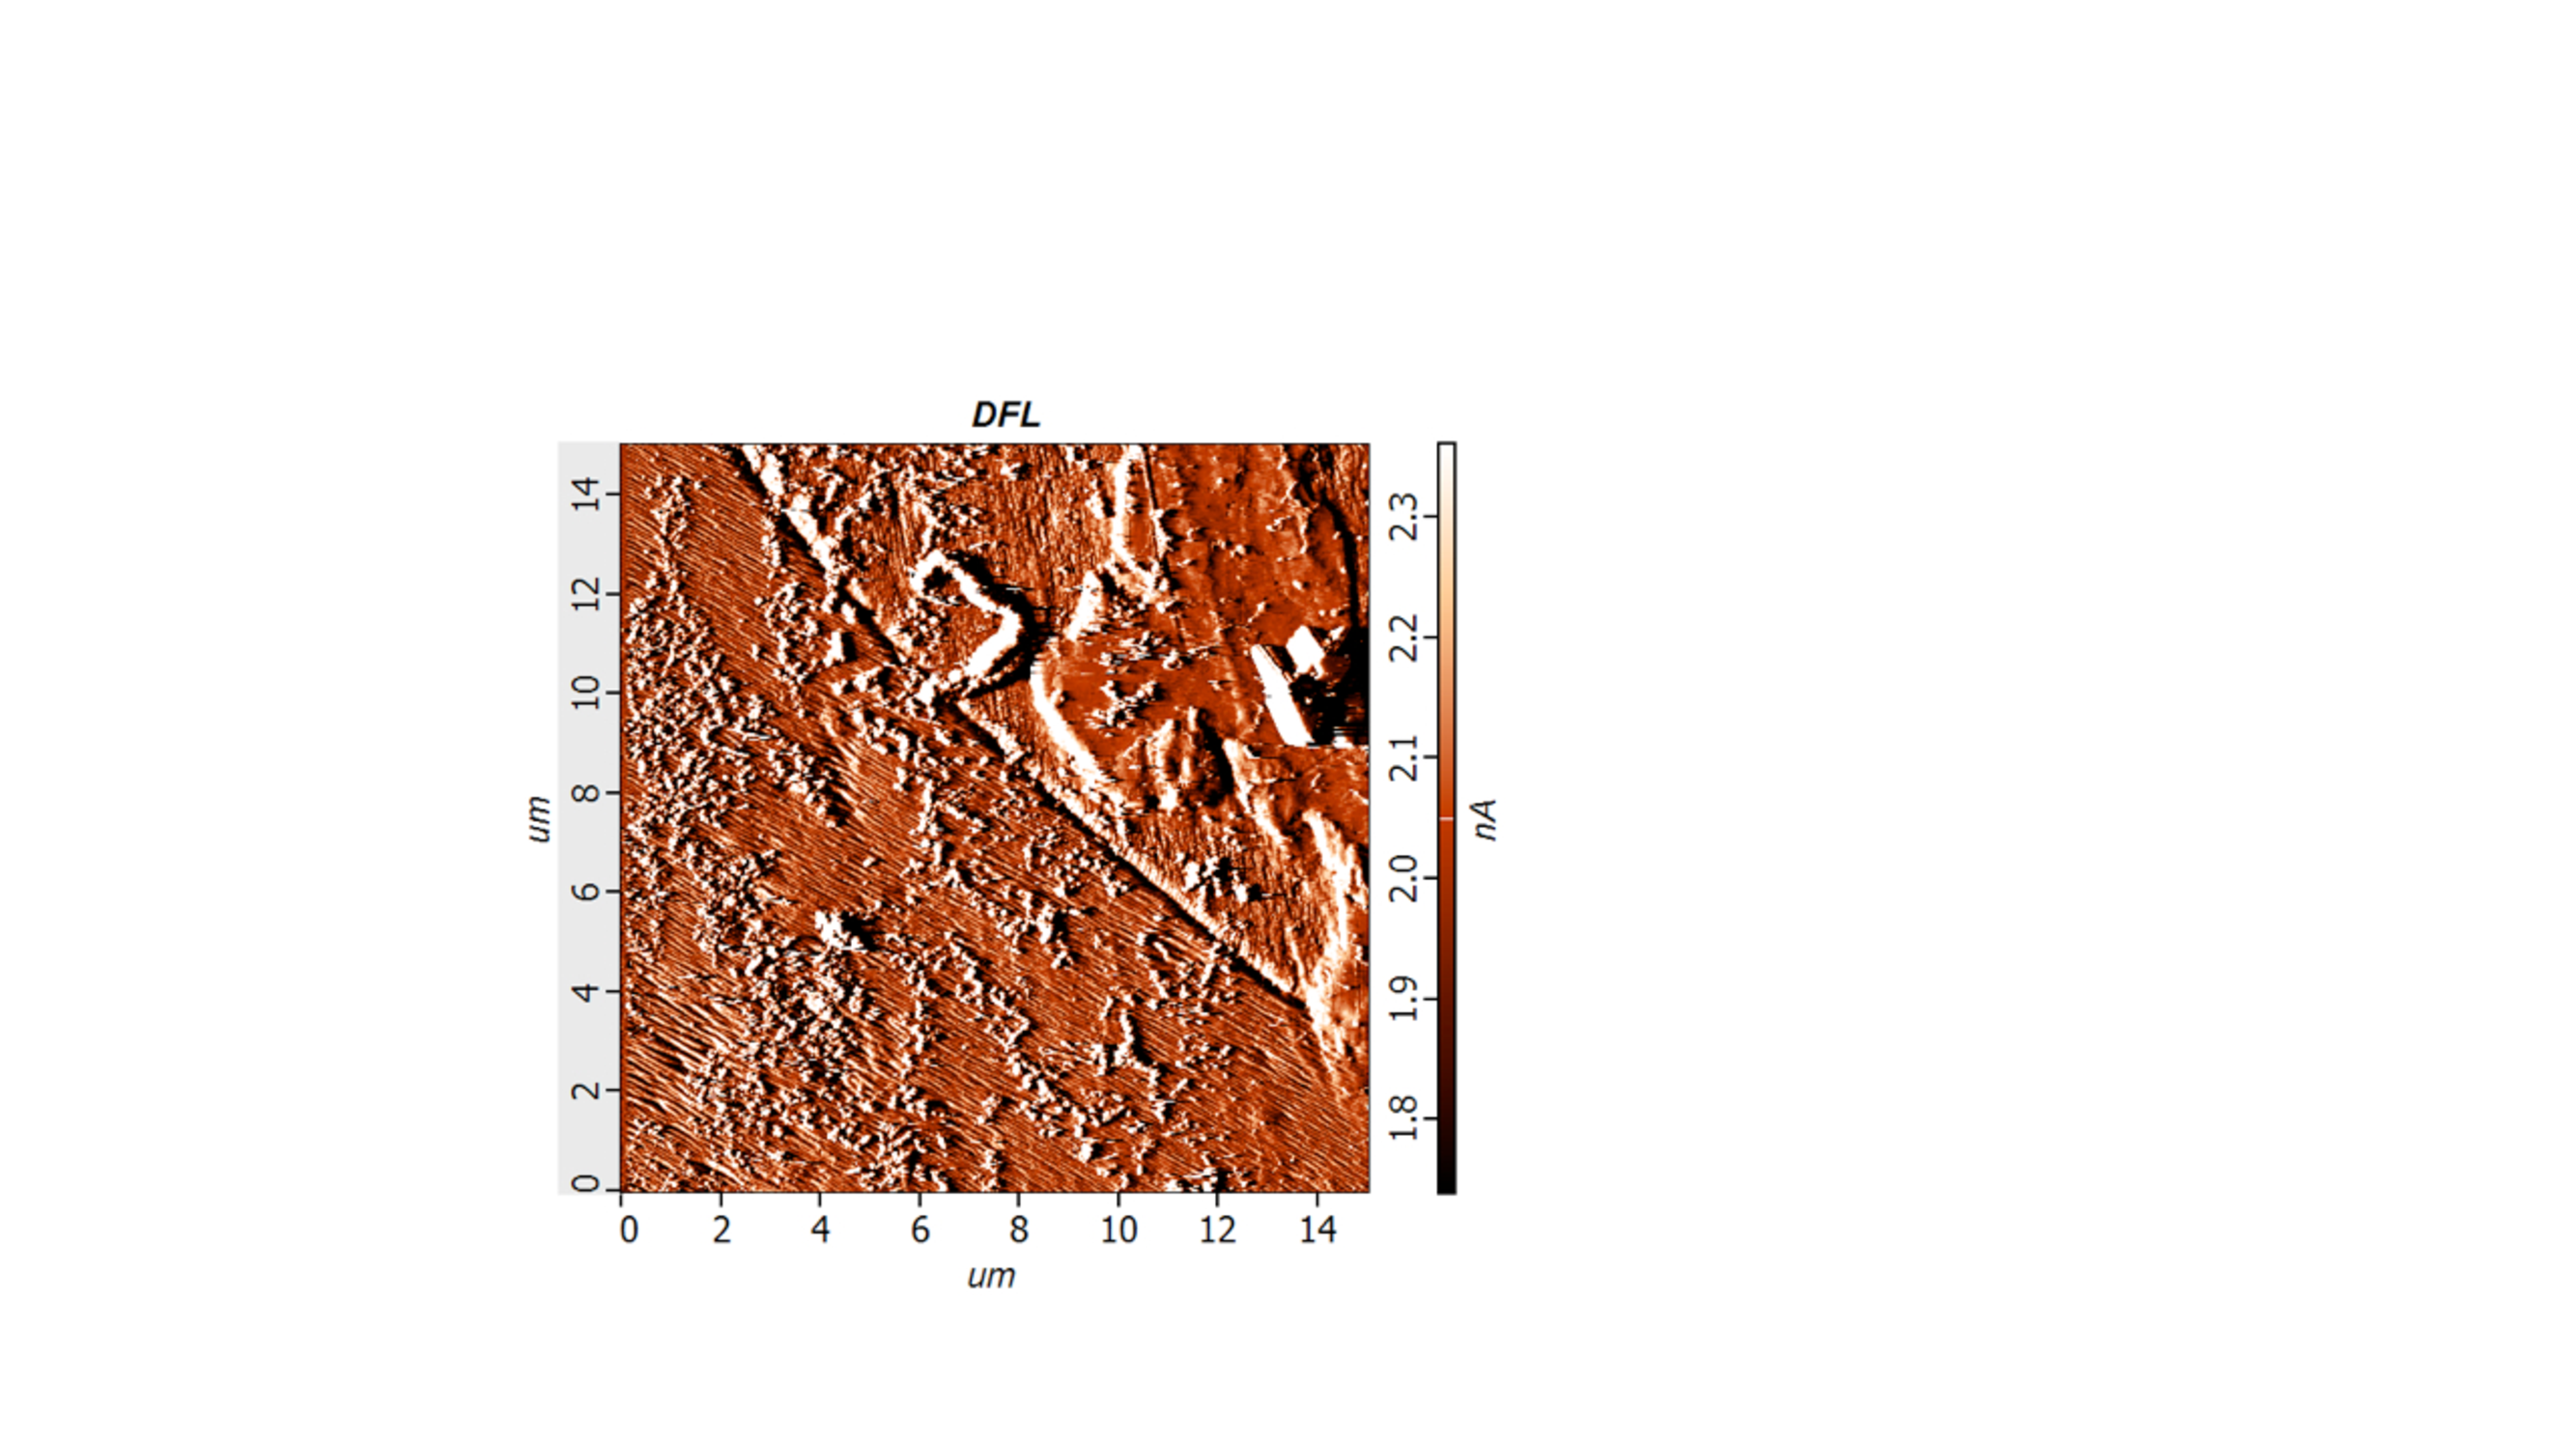
\includegraphics[width=0.5\textwidth]{btouv.pdf}
\caption[AFM deflection image reaction on \SI{7}{\nano\meter} thick \ce{Fe2O3} film]{AFM deflection image of the surface of a \SI{7}{\nano\meter} thick \ce{Fe2O3} film on \ce{BaTiO3} after reaction with \ce{AgNO3} under UV light. The heterostructure does not show the same behavior as \ce{TiO2}/\ce{BaTiO3} heterostructures.}
\label{fig:btouv} % Figure 6.8
\end{center}
\end{figure}
No domain-specific spatially-selective reactivity is observed in these micrographs. No other examined areas of the sample showed spatially selective reactivity.

Burbure observed that spatially-selective reactivity could be turned off by increasing the thickness of the film, or by increasing the density of charge carriers in the film. It was hypothesized that both of these factors resulted in a completely screened space charge-region within the film. By increasing the film thickness without changing the charge carrier concentration in the film, eventually the film is thicker than the space-charge region in the film. The film is able to completely screen the electric fields arising from the buried ferroelectric interface, and spatially-selective reactivity no longer occurs. As the width of the space charge region is inversely proportional to the carrier concentration in the film. If the carrier concentration in the film is increased, the space-charge width is decreased, and even very thin films are able to completely screen the fields from ferroelectric polarization. A possible explanation for the lack of spatially-selective reactivity on the \ce{Fe2O3} films is the possibility of a much higher film charge carrier density than for \ce{TiO2} films. If this is the case, it is possible even the \SI{7}{\nano\meter} \ce{Fe2O3} film could be completely screening the ferroelectric polarization. 

For all \ce{Fe2O3} films on \ce{BaTiO3} substrates, spatially selective photochemical reactivity was never observed. This suggests that \ce{Fe2O3} films behave fundamentally differently than \ce{TiO2} films on the same substrates. Film quality and interface quality are possible explanations for the differing behavior. Chemical similarity between \ce{TiO2} and \ce{BaTiO3} could result in higher quality films, with fewer defects in the film. As defects are scattering centers, acting as obstacles to charge carrier transport, a lower quality film would hinder the movement of charge carriers from the substrate to the surface of the film. The results on \ce{Fe2O3} film growth presented earlier in this chapter show that a significant fraction of the substrate grains nucleated epitaxial film grains of high enough crystallinity for automated EBSD indexing. This suggests that poor film quality is not the explanation for the lack of selective reactivity. The nature of the interface between the film and substrate is not known. If the interface is composed of a thin layer of highly disordered material, this could prevent charge carriers from leaving the substrate and entering the film. This would explain the overall low levels of reactivity observed, and the lack of selective reactivity. A final explanation would be that the charge carrier concentration in the film is high enough that even a \SI{5}{\nano\meter} film completely screen the charge of the ferroelectric substrate. Currently, the charge carrier density of the \ce{Fe2O3} films is unknown. An accurate measurement of the film charge carrier density will help determine whether this is the cause of the lack of spatially-selective reactivity. Experiments testing the charge carrier concentration of the hematite films in this work are proposed in \S \ref{sec:ch8plan}.


\subsection{Grain-selective Reactivity}
\label{subsec:ch6grain}


While testing for selective reactivity resulting from the ferroelectric domains of the substrate, and it was observed that certain film grains of an \ce{Fe2O3} film on polycrystalline \ce{BaTiO3} were much more reactive than other grains. Figure \ref{fig:btoreacted} shows a screen capture of the optical viewing system taken during AFM measurements of the film surface after reaction with \ce{AgNO3}.
\begin{figure}[htbp]
\begin{center}
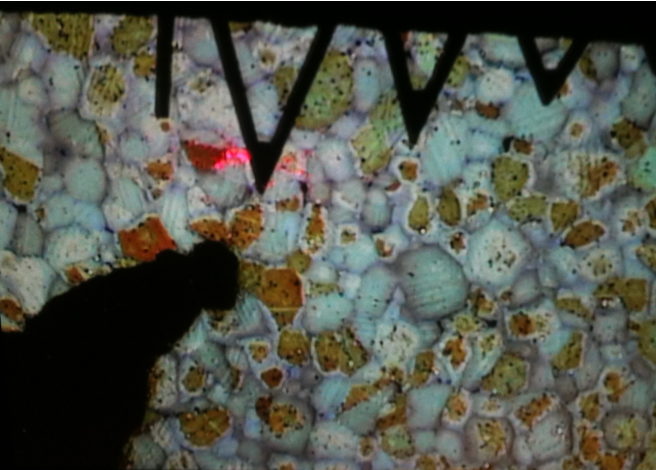
\includegraphics[width=\textwidth]{btoreacted.pdf}
\caption[Optical image showing grain selective reactivity]{Screenshot of the optical viewing system of an AFM showing grain selective reactivity. Brown grains correspond to regions with a high concentration of photochemical reaction product on the surface.}
\label{fig:btoreacted} % Figure 6.9
\end{center}
\end{figure}
Some grains appear brown in the image. These grains correspond to grains with a high amount of reaction product on the surface. After the surface of the sample was cleaned, as shown in Figure \ref{fig:btoclean}, all the grains appeared similar, and the reaction product was no longer visible.
\begin{figure}[htbp]
\begin{center}
\includegraphics[width=\textwidth]{btoclean.pdf}
\caption[Area of the surface depicted in Figure \ref{fig:btoreacted} after cleaning]{The same area of the surface depicted in Figure \ref{fig:btoreacted} after cleaning, showing that the brown material was indeed reaction product, and could be cleaned from the surface.}
\label{fig:btoclean} % Figure 6.10
\end{center}
\end{figure}
A difference in photochemical reactivity high enough to be so easily observed in the optical viewing system of the AFM has not typically been observed in previous experiments on other material systems.

The area of the sample shown in this figure corresponds to the same area of the sample used to determine the orientation relationships between the substrate grains and the film grains. As a result, the orientations of the substrate and film grains are known. Figure \ref{fig:btooverlay} shows the optical microscopy image overlaid on the inverse pole map, clearing showing that the grains with a consistent, easily indexed orientation were the grains with the high photochemical activity.
\begin{figure}[htbp]
\begin{center}
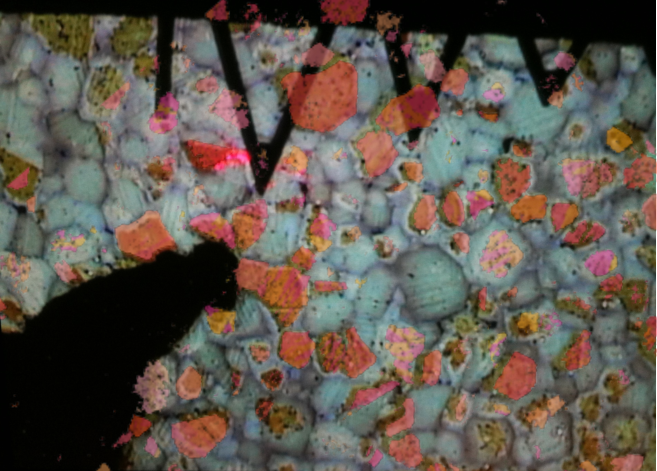
\includegraphics[width=\textwidth]{btooverlay.pdf}
\caption[Inverse pole map overlaid on the image from Figure \ref{fig:btoreacted}]{Inverse pole map from Figure \ref{fig:orientationmaps}(b) overlaid on the image from Figure \ref{fig:btoreacted}. In many cases, the grains that showed high photochemical activity are also grains that nucleated high quality \ce{Fe2O3} films.}
\label{fig:btooverlay} % Figure 6.11
\end{center}
\end{figure}
What is striking is that the grains with high photochemical activity correspond to grains that indexed well during the EBSD scan. 

Two explanations are proposed for the increased reactivities of these grains. All of the film grains with high reactivity are oriented near the (0001) direction, with the c-axis pointing out of the sample surface. The substrate grains are predominately (111) and (011) oriented grains. All of the film grains that did not demonstrate high reactivity were also grains that were not indexed during the automated EBSD process. This suggests that the grains are either amorphous, or polycrystalline with grain sizes much smaller than the electron probe. 

It has been demonstrated previously that c-axis oriented \ce{Fe2O3} supported on single crystal (111) oriented \ce{SrTiO3} substrates are highly reactive. The highly active grains in this sample show the same orientation relationship, and have similar planes oriented out of the surface. If the charged interface hypothesis presented in Chapter \ref{ch:thinfilmreactivity} is correct, this could be the same mechanism responsible for the highly reactive nature of these grains. The (001) perovskite surface is neutral, existing as termination of BaO and \ce{TiO2} layers. The (111) and (110) surfaces of \ce{BaTiO3} are polar, consisting of (111) terminations here, and BaTiO and \ce{O2} layers for the (110) surface. The fact that the highly active film grains are all supported on substrate grains with orientations near the polar (111) or (110) surface suggests that the polar surface is responsible for the increased reactivity.

However, as described previously, grains with poor crystallinity and a high concentration of structural defects such as grain boundaries and dislocations are associated with decreased photochemical reactivity. The grains that were not highly active were also the grains believed to be of poor crystalline quality. They were not automatically indexed during EBSD scanning, and manual inspection of the EBSD pattern quality for these locations showed that patterns were extremely poor or non existent for these areas of the sample. As a result, these experiments are not conclusive evidence that the charged surface hypothesis is solely responsible for the differing reactivities of the grains in this sample. 


\section{Conclusions for Polycrystalline Substrates}
\label{sec:ch6conclusions}


The orientation relationship for \ce{Fe2O3} films on perovskite \ce{BaTiO3} substrates was determined. Single film grains, or in some cases twinned film grains, grew on the entire area of single substrate grains located away from the (001) cubic orientation. These film grains were oriented near the hexagonal (0001) orientation. It was determined that the film [001] direction was parallel to the substrate [111] direction, even when the [111] direction was located far away from normal to the sample surface. The substrate [1\={1}0] direction also determined to be parallel to the film [210] direction, even when these directions did not lie in the plane of the sample. 

Heterostructures of \ce{Fe2O3} films on polycrystalline \ce{BaTiO3} substrates do not show the same photochemical behavior as for \ce{TiO2} films on \ce{BaTiO3} substrates. No spatially selective reactivity corresponding to ferroelectric domains was observed, even for very thin films. High reactivity was observed on film grains with films near the (0001) orientation, though whether this is because of the film orientation, substrate surface polarity, or higher crystalline quality of the film is unknown.